\section{Account structure}\label{sec:account}

\subsection{Definitions}

\begin{defn}[Account]\label{def:account}
An account $\zeta$ is a list of properties that defines the owner of an asset $\theta$ in the ledger.
\end{defn}

Specifically an account is composed by a set of attributes, represented by an address and incorporates a set of functions that apply on the assets that it owns. These functions include moving an asset to a different account, i.e. \textbf{payment}, or taking part in Proof-of-Stake protocol-related actions as the rightful asset owner, i.e. \textbf{staking}.

\begin{defn}[Account attribute]\label{def:attribute}
An attribute $\delta$ is a string $\delta \in \Delta, \Delta \subseteq \{0, 1\}^\kappa$ that identifies a property of the account.
\end{defn}

An example of an account attribute is the payment key $K^p$. Specifically, $\delta = K^p$, $\Delta$ is the range of the key generation function and the account property that $K^p$ identifies is \textit{the ability to spend the assets in the account}.

\begin{defn}[Account attribute list]\label{def:attributelist}
The account attribute list $\mathcal{D}$ is the list of all attributes $\mathcal{D} = [{\delta}_1 \in {\Delta}_1, {\delta}_2 \in {\Delta}_2, \ldots, {\delta}_m \in {\Delta}_m]$ of an account. For any two accounts ${\zeta}_1, {\zeta}_2$ with attribute lists ${\mathcal{D}}_1, {\mathcal{D}}_2$ respectively it holds: ${\mathcal{D}}_1 = {\mathcal{D}}_2 \iff {\zeta}_1 \equiv {\zeta}_2$.
\end{defn}

\begin{defn}[Account address]\label{def:address}
The address $\alpha$ of an account $\zeta$ is a string $\alpha \in \{0, 1\}^\mu$ that uniquely represents $\zeta$.
\end{defn}

For the rest of the paper we will use the address $\alpha$ to refer to account $\zeta$.

\begin{defn}[Address generation function]\label{def:addressgen}
The address generation function $f : {\Delta}_1 \times \ldots \times {\Delta}_m \rightarrow \{0, 1\}^\mu$ is a function that, given an account attribute list, outputs an address.
\end{defn}

The implementation of $f$ and the attributes in $\mathcal{D}$ depend on the specifications of the protocol.

\begin{defn}[Transaction]\label{def:transaction}
A transaction $\tau$ is the output of any function $g$ applied on an account $\zeta$ and an asset $\theta$ in the ledger: $\tau = g(\theta, \zeta)$. $\tau$ is \textbf{valid} iff $\theta$ is owned by $\zeta$.
\end{defn}

\subsection{Account attributes}

We now define some fundamental account attributes, specifically the keypair and the hierarchical wallet tag.

\begin{defn}[Account key pair]\label{def:keypair}
The account key pair $K$ is a pair of keys, the payment key $K^p$ and the staking key $K^s$.
\end{defn}

$K^p$ is used for payments, i.e. transferring the coins that are held by the account to a different account. $K^s$ is used for staking, i.e. taking part in the Proof-of-Stake protocol, either as a committee member or a slot leader, or delegating the stake to a different staking key.

\begin{defn}[Hierarchical wallet tag]\label{def:hierarchical_tag}
The hierarchical wallet tag $ht$ is a string that is used to identify whether an address is part of a hierarchical wallet.
\end{defn}

\begin{defn}[Spending list]\label{def:spending_part}
The spending list $S$ of an account is a list of attributes that are revealed when a transaction is created that spends from the account. The hash of the spending set is $H_s$.
\end{defn}

We include all attributes in the spending part of the tree to avoid a spending malleability attack. In such scenario, an attacker $A$ wishes to send some money to an honest receiver $B$, so she obtains an address $\alpha$ from $B$. She is successful if she is able to change $\alpha$ and create an address $\alpha'$, so that the balance in $\alpha'$ can be spent using the same payment key that was used to create $\alpha$, whilst some other attribute of $\alpha$, e.g. the staking key, has been replaced with an adversarial one.

\subsubsection{Public attributes}

Public attributes are attributes that need be publicly visible in the address. Specifically, they must exist in plaintext form in the address and can be recognized and used by the system automatically in order to complete protocol-related functionalities.

A public attribute is present in both the address and the spending set $S$.

Examples of public attributes are the delegation pointer, in case of an pointer account, or the hierarchical wallet tag.

\subsubsection{Private attributes}

These attributes become public only when a transaction is published that spends the entire account's balance.

Private attributes are present only in the spending set $S$ and are revealed only when a spending transaction is made.

The primary example of such an attribute is the payment key $K^p$.

\subsection{Address structure}

The address of an account is the concatenation of the root of the tree that identifies the account with the public attributes of the account.

We now describe the structure of the address of three types of accounts, the \textbf{base} account, the \textbf{pointer} account and the \textbf{enterprise} account. These types of accounts differ on the way the stake that they hold is delegated, as well as the structure of the address that represents them.

\subsubsection{Base account}\label{subsubsec:base_account_v2}

A base account is managed by the payment key $K^p$. This account is formed by this key along with the public attributes that are the hash of a staking key $K^s$, which we call delegation hash $dh$, and the hierarchical tag $ht$.

The core part of the address is the root of the attribute tree. This is the hash of all attributes in the spending set, i.e. the payment key and the public attributes.

The stake that is held by the base account is delegated to the staking key $K^s$. Therefore the account links to the staking information, which is in this case the staking key.

The attributes and the address structure of a base account can be seen in Figure \ref{fig:base_account_v2}.

\begin{figure}
  \begin{center}
    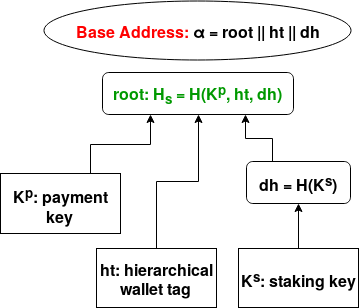
\includegraphics[width=230pt]{figures/base_account_v2.png}
  \end{center}
  \caption{The base account.}
  \label{fig:base_account_v2}
\end{figure}

\subsubsection{Pointer account}\label{subsubsec:pointer_account}

A pointer account is managed by a single payment key $K^p$. Therefore, the owner of such account can only complete one action, that is spending the balance of the account, whereas all other actions that pertain to the Proof-of-Stake protocol are completed by the system.

The core part of the address is again the root of the attribute tree. However, in this case this part is just the hash of all of the account's attributes, i.e. it is the hash of the spending set defined in \ref{def:spending_part}. The rest of the address consists of the hierarchical wallet tag and the delegation pointer.

The delegation pointer is used to identify the staking key that the stake in the account is delegated to. Specifically, the pointer points to a transaction that contains a registration certificate for a staking key that has been published on the blockchain. That way the delegate key for the pointer address is the one defined in the certificate that the account points to and, given that this information is included in the address in plaintext form, the stake in the pointer account is delegated to the registered staking key. Similarly to the base account described above, the pointer account links to the staking information.

The attributes and the address structure of a pointer account can be seen in Figure \ref{fig:pointer_account}.

\begin{figure}
  \begin{center}
    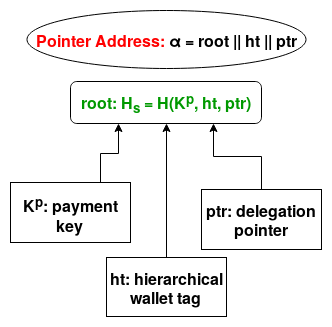
\includegraphics[width=210pt]{figures/pointer_account.png}
  \end{center}
  \caption{The pointer account.}
  \label{fig:pointer_account}
\end{figure}

\subsubsection{Enterprise account}\label{subsubsec:enterprise_account_plain}

An enterprise account is an account managed by a payment key $K^p$. The stake in this account is not delegated to any staking key and is excluded from all protocol operations, like the block creation. An enterprise account is identified by the enterprise identifier $\epsilon$, which is a public attribute of the account.

The address structure of an enterprise account can be seen in Figure \ref{fig:enterprise_account_plain}.

\begin{figure}
  \begin{center}
    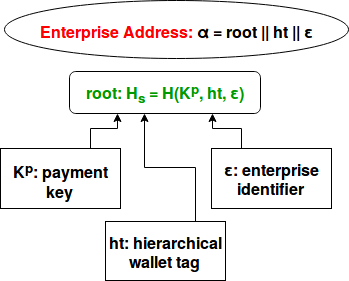
\includegraphics[width=210pt]{figures/enterprise_account_plain.png}
  \end{center}
  \caption{The enterprise account.}
  \label{fig:enterprise_account_plain}
\end{figure}
